\documentclass{beamer}
\usepackage{amsmath}
\usepackage[utf8]{inputenc}
\usepackage{hyperref}
\usepackage{multicol}
\usepackage{hyperref}

\inputencoding{utf8}

\mode<presentation> {
    \usetheme{Madrid}
}

\usepackage{graphicx}
\usepackage{booktabs}

\title[Matematica discreta]{Matematica discreta elemental}
\author{Ernesto Rodriguez}
\institute{
    Universidad del Itsmo \\
    \medskip \textit{erodriguez@unis.edu.gt}
}

\date[\today]{}

\begin{document}

\begin{frame}
\titlepage
\end{frame}

\begin{frame}
\frametitle{Principios basicos}
\begin{itemize}
    \item{Los numeros son representaciones simbolicas de cantidades.}
    \item{Se pueden representar de muchas formas}
    \item{Consideremos la m\'as basica:\\
        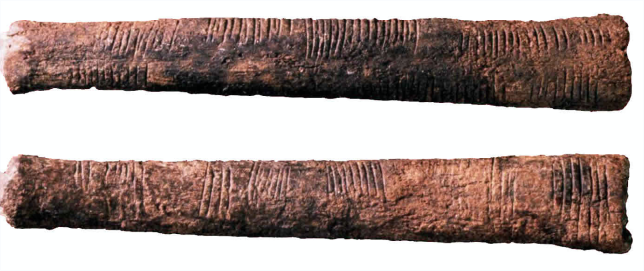
\includegraphics[width=6cm]{numbers.png}
    }
    \item{Se utilizan marcas en una superficie para contar.}
    \item{Por ejemplo: ``////'' significa cuatro.}
\end{itemize}
\end{frame}

\begin{frame}
    \frametitle{Construccion Algoritmica}
    Se utilizaran dos reglas para construir los numeros:
    \begin{itemize}
        \item{{\bf regla-$o$} el espacio vacio (' ') es un numero.}
        \item{{\bf regla-$s$} se puede construir un numero nuevo colocando una marca
        (``/'') despes de un numero existente.}
        \item{{\bf Ejemplo:} El numero ``////'' se produce mediante la aplicaci\'on de la
        regla-$o$ y cuatro aplicaciones de la regla-$s$}
        \item{Los numeros construidos mediante estas reglas se conocen como: \emph{Numeros unarios naturales}}
    \end{itemize}
\end{frame}

\begin{frame}
\frametitle{M\'as formalidad}
\begin{itemize}
    \item{{\bf Definici\'on}: Un numero natural unario es el \emph{sucesor} (\emph{predecesor})
    si se puede construir al agregar (quitar) una marca -- la regla-$s$ produce los sucesores.}
    \item{{\bf Ejemplo:} /// es el sucesor de // y // el predecesor de ///}
\end{itemize}
\end{frame}

\begin{frame}
    \frametitle{Axiomas de Peano}
    \begin{itemize}
    \item{{\bf Aximoa (P1): } ' ' (llamado cero) es un numero unario natural}
    \item{{\bf Axioma (P2): } Todo numero natural unario tiene un sucesor que es diferente
    a el}
    \item{{\bf Axioma (P3): }El cero no es el sucesor de ning\'un numero natural unario}
    \item{{\bf Axioma (P4): }Diferentes numeros naturales unarios tienen diferentes sucesores}
    \item{{\bf Axioma (P5: Inducci\'on): }Todos los numeros naturales unarios tienen una propiedad
    $P$ si:
    \begin{enumerate}
        \item{\emph{cero} tiene la propiedad $P$}
        \item{El sucesor de todo numero con la propiedad $P$ tambi\'en tiene la propiedad $P$.}
    \end{enumerate}
    \item{{\bf Pregunta: } ¿Por que es necesaria tanta formalidad?}
    \item{``Este es el precio que hay que pagar para estar absolutamente seguro'' -- Bernard Russel}
    }
\end{itemize}
\end{frame}

\begin{frame}
    \frametitle{Razonamiento sobre Numeros Naturales Unarios}
    \begin{itemize}
        \item{Los \emph{axiomas de Peano} nos permiten razonar acerca de los numeros naturales}
        \item{{\bf Definici\'on}: Un \emph{axioma} es un enunciado sobre objetos matematicos que
        asumimos ser cierto}
        \item{Un \emph{teorema} es un enunciado sobre objetos matematicos que sabemos que es cierto}
        \item{Razonamos acerca de los numeros naturales infiriendo teoremas a partir de axiomas u
        otros teoremas. Ej:
        \begin{enumerate}
            \item{' ' es un numero natural unario (axioma P1)}
            \item{/ es un numero natural unario (axioma P2 y 1)}
            \item{// es un numero natural unario (axioma P2 y 2)}
        \end{enumerate}
        }
        \item{Una sequencia de inferencias es una \emph{demostraci\'on} del ultimo
        enunciado.}
    \end{itemize}
\end{frame}

\begin{frame}
    \frametitle{M\'as teoremas y demostraciones}
    \begin{itemize}
        \item{{\bf Teorema: }////////// es un numero natural unario}
        \item{{\bf Teorema: }/// es diferente de //}
        \item{{\bf Teorema: }///// es diferente de //}
        \item{{\bf Teorema: }Existe un numero natural unario que es sucesor de ///}
        \item{{\bf Teorema: }Existen al menos 7 numeros naturales unarios}
        \item{{\bf Teorema: }Todo numero natural unario es cero o el sucesor de otro
        numero natural unario}
    \end{itemize}
\end{frame}

\begin{frame}
    \frametitle{Inducci\'on para los numeros naturales unarios}
    \begin{itemize}
        \item{{\bf Teorema: }Todo numero natural unario es cero o el sucesor de
        otro numero}
        \item{Demostraci\'on mediante el axioma P2:
        \begin{enumerate}
            \item{Se considera la propiedad $p$ que dice ``es cero o sucesor'' y se verifican los
            requisitos.}
            \item{El numero ' ' es cero, por lo que cumple con $p$}
            \item{Considerar un numero natural unario arbitrario $n$ que cumple con $p$}
            \item{El numero $n$ tiene un sucesor llamado $s(n)$ (P2).}
            \item{Dado que $n$ fue arbitrario, mediate P5 concluimos que todo
            numero natural unario cumple con $p$.}
        \end{enumerate}
        }
    \end{itemize}
\end{frame}

\begin{frame}
    \frametitle{Notaci\'on}
    \begin{itemize}
        \item{Es permitido nombrar un numeor natural unario arbitrario mediante una variable ($n,m,l,k,n_1,n_2$)}
        \item{Representamos los numeros mediante la aplicaci\'on de reglas que los construye: ////
        se representa como $s(s(s(s(o))))$}
        \item{{\bf Definici\'on: }Introduciomos alg\'unas abreviaciones:
        \begin{itemize}
            \item{Se abrevia a $o$ o ' ' mediante el simbolo '0'}
            \item{Se abrevia a $s(o)$ y / mediante el simbolo '1'}
            \item{Se abrevia a $s(s(o))$ y // mediante '2'}
            \item{...}
        \end{itemize}
        }
        \item{$\mathbb{N}_1$ representa al conjunto de todos los numeros naturales}
    \end{itemize}
\end{frame}

\begin{frame}
    \frametitle{El Teorema Domino}
    \begin{itemize}
        \item{{\bf Teorema: }Consideremos una secuencia $S_0,S_1,...$ de dominos, tal
        que cada numero natural unario $n$ comple con:
        \begin{itemize}
            \item{La distancia entre $S_n$ y $S_{s(n)}$ es menor que la altura de $S_n$}
            \item{$S_n$ es m\'as alto que ancho, por ente inestable}
            \item{$S_n$ y $S_{s(n)}$ tienen el mismo peso}
            \item{Todos los dominoes $S_n$ se encuentran en una linea recta}
        \end{itemize}
        }
        \item{{\bf Teorema: }Si $S_0$ cae en la direccion de $S_1$, todos los dominos caen}
    \end{itemize}
    \begin{center}
        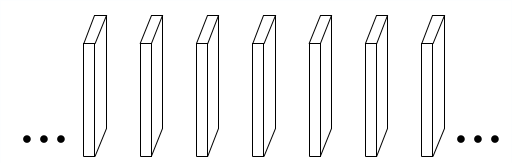
\includegraphics[width=6cm]{dominoes.png}
    \end{center}
\end{frame}

\begin{frame}
    \frametitle{La Inducci\'on de Domino}
    \begin{itemize}
        \item{{\bf Demostraci\'on: }Demostramos el teorema mediante inducci\'on
        sobre $n$ con la propiedad $P$ que dice: ``$S_n$ cae en la direcci\'on de $S_{s(n)}$''}
        \item{Hay que considerar dos casos:
            \begin{itemize}
                \item{{\bf Caso base: } $n$ es cero
                \begin{enumerate}
                    \item{Asumimos que $S_0$ se empuja en la direcci\'on de $S_1$ por lo cual cae}
                \end{enumerate}
                }
                \item{{\bf Caso inductivo: }$n$ es un numero natural unario arbitrario
                \begin{enumerate}
                    \item{$n=s(m)$ para algun numero natural unario $m$ (P2)}
                    \item{Asumimos que $P$ se mantiene, por lo cual $S_m$
                    cae en la direcci\'on de $S_{s(m)}$}
                    \item{Sabemos que $S_m$ empuja a $S_{s(m)}$ en la direccion opuesta que
                    cayo ya que la distancia entre ambos es menor que la altura de $S_m$ y la
                    segunda ley de newton}
                    \item{Debido a que $S_{s(m)}$ tiene el mismo peso que $S_m$ y es inestable,
                    debe caer en la direcci\'on opuesta que cayo $S_m$}
                \end{enumerate}
                }
            \end{itemize}
        }
    \end{itemize}
\end{frame}

\end{document}